% ============================================================================
%  CHAPTER 24 — COMPREHENSIVE THREAT MODELING AND SECURITY ANALYSIS
% ============================================================================
\chapter{Comprehensive Threat Modeling and Security Analysis}
\label{ch:threat-model}

\epigraph{Security is not a product.  It is a process.}{Bruce Schneier}

This chapter applies systematic threat-modeling methodologies to the
PQC Secure MAVLink Tunnel, identifies attack surfaces, constructs
attack trees, evaluates residual risks, and maps every threat to its
corresponding mitigation in the codebase.

% ────────────────────────────────────────────────────────────────────────────
\section{Methodology}
\label{sec:tm-methodology}

We combine three complementary frameworks:

\begin{enumerate}
  \item \textbf{STRIDE} (Microsoft)---categorises threats by type
        (Spoofing, Tampering, Repudiation, Information Disclosure,
        Denial of Service, Elevation of Privilege).
  \item \textbf{Attack Trees} (Schneier)---hierarchical decomposition
        of adversary goals into sub-goals and leaf-level attack steps.
  \item \textbf{DREAD} scoring---quantifies risk on five axes (Damage,
        Reproducibility, Exploitability, Affected Users, Discoverability),
        each scored 1--10.
\end{enumerate}

\paragraph{Adversary Model.}
We consider four adversary classes, ordered by increasing capability:

\begin{longtable}{c l p{6cm}}
  \caption{Adversary classes.}
  \label{tab:tm-adversaries} \\
  \toprule
  \textbf{Class} & \textbf{Name} & \textbf{Capabilities} \\
  \midrule
  \endfirsthead
  \bottomrule
  \endfoot

  $\mathcal{A}_1$ & Passive Eavesdropper & Captures all network traffic (WiFi monitor mode).
    Cannot inject or modify packets.  Can store ciphertext for future
    quantum decryption (``harvest now, decrypt later''). \\
  $\mathcal{A}_2$ & Active Network Attacker & All of $\mathcal{A}_1$ plus: inject, drop, reorder, replay, and modify
    packets.  Equivalent to a Dolev--Yao attacker on the network. \\
  $\mathcal{A}_3$ & Compromised Endpoint & All of $\mathcal{A}_2$ plus: read/write access to one endpoint
    (drone \emph{or} GCS, not both).  Can extract keys, modify binaries,
    access configuration files. \\
  $\mathcal{A}_4$ & Quantum Adversary & All of $\mathcal{A}_1$ plus: access to a cryptographically
    relevant quantum computer (CRQC).  Can run Shor's algorithm on
    stored ciphertext.  Cannot yet operate in real time. \\
\end{longtable}

% ────────────────────────────────────────────────────────────────────────────
\section{System Decomposition}
\label{sec:tm-decomposition}

\subsection{Trust Boundaries}

Figure~\ref{fig:tm-trust-boundaries} shows the four trust boundaries
in the system.

\begin{figure}[H]
  \centering
  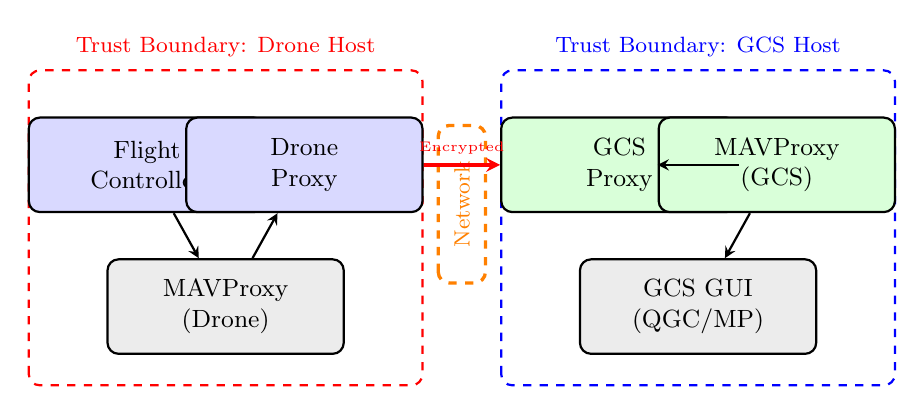
\begin{tikzpicture}[
    box/.style={draw, thick, rounded corners, minimum width=3cm,
                minimum height=1.2cm, font=\small, align=center},
    boundary/.style={draw, dashed, thick, rounded corners, #1},
    arrow/.style={->, thick, >=stealth},
  ]
    % Drone boundary
    \draw[boundary=red] (-5.5, -1.8) rectangle (-0.5, 2.2);
    \node[font=\footnotesize, red] at (-3, 2.5) {Trust Boundary: Drone Host};
    
    \node[box, fill=blue!15]  (fc)    at (-4, 1)  {Flight\\Controller};
    \node[box, fill=blue!15]  (dprox) at (-2, 1)  {Drone\\Proxy};
    \node[box, fill=gray!15]  (dmav)  at (-3, -0.8) {MAVProxy\\(Drone)};
    
    % GCS boundary
    \draw[boundary=blue] (0.5, -1.8) rectangle (5.5, 2.2);
    \node[font=\footnotesize, blue] at (3, 2.5) {Trust Boundary: GCS Host};
    
    \node[box, fill=green!15] (gprox) at (2, 1)   {GCS\\Proxy};
    \node[box, fill=green!15] (gmav)  at (4, 1)   {MAVProxy\\(GCS)};
    \node[box, fill=gray!15]  (gui)   at (3, -0.8) {GCS GUI\\(QGC/MP)};
    
    % Network boundary
    \draw[boundary=orange, very thick] (-0.3, -0.5) rectangle (0.3, 1.5);
    \node[font=\footnotesize, orange, rotate=90] at (0, 0.5) {Network};
    
    % Arrows
    \draw[arrow] (fc) -- (dmav);
    \draw[arrow] (dmav) -- (dprox);
    \draw[arrow, red, very thick] (dprox) -- node[above, font=\tiny] {Encrypted} (gprox);
    \draw[arrow] (gprox) -- (gmav);
    \draw[arrow] (gmav) -- (gui);
  \end{tikzpicture}
  \caption{Trust boundaries and data flow.  The red thick arrow
           crosses the untrusted network boundary.}
  \label{fig:tm-trust-boundaries}
\end{figure}

\subsection{Data Flow Diagram (DFD)}

\begin{longtable}{c l l l p{3cm}}
  \caption{Data flows across trust boundaries.}
  \label{tab:tm-data-flows} \\
  \toprule
  \textbf{ID} & \textbf{From} & \textbf{To} & \textbf{Protocol} & \textbf{Data} \\
  \midrule
  \endfirsthead
  \bottomrule
  \endfoot

  DF1 & FC              & MAVProxy (D) & Serial/UDP & MAVLink v2 (cleartext) \\
  DF2 & MAVProxy (D)    & Drone Proxy  & UDP (local) & MAVLink v2 (cleartext) \\
  DF3 & Drone Proxy     & GCS Proxy    & TCP         & ServerHello / ClientReply \\
  DF4 & Drone Proxy     & GCS Proxy    & UDP         & EncryptedDatagram \\
  DF5 & GCS Proxy       & Drone Proxy  & UDP         & EncryptedDatagram \\
  DF6 & GCS Proxy       & MAVProxy (G) & UDP (local) & MAVLink v2 (cleartext) \\
  DF7 & MAVProxy (G)    & GCS GUI      & TCP/UDP     & MAVLink v2 (cleartext) \\
  DF8 & Drone Scheduler & GCS Scheduler & TCP        & JSON commands (cleartext) \\
\end{longtable}

\subsection{Entry Points}

\begin{longtable}{l l l p{4cm}}
  \caption{System entry points.}
  \label{tab:tm-entry-points} \\
  \toprule
  \textbf{ID} & \textbf{Port} & \textbf{Protocol} & \textbf{Description} \\
  \midrule
  \endfirsthead
  \bottomrule
  \endfoot

  EP1 & 46000  & TCP  & Handshake listener (GCS mode). \\
  EP2 & 47001  & UDP  & Encrypted data ingress (drone). \\
  EP3 & 47002  & UDP  & Encrypted data ingress (GCS). \\
  EP4 & 48080  & TCP  & Scheduler command server (GCS). \\
  EP5 & 14550  & UDP  & MAVProxy telemetry (local only). \\
  EP6 & ---    & File & Configuration files (\texttt{settings.json}). \\
  EP7 & ---    & File & Cryptographic key files (\texttt{keys/*.pub}, \texttt{keys/*.key}). \\
  EP8 & ---    & Env  & Environment variables (\texttt{SECDRONE\_*}). \\
\end{longtable}

% ────────────────────────────────────────────────────────────────────────────
\section{STRIDE Analysis}
\label{sec:tm-stride}

\begin{longtable}{l l l c p{4.5cm}}
  \caption{STRIDE threat enumeration.}
  \label{tab:tm-stride} \\
  \toprule
  \textbf{ID} & \textbf{STRIDE} & \textbf{Target} & \textbf{Adv.} & \textbf{Description} \\
  \midrule
  \endfirsthead
  \toprule
  \textbf{ID} & \textbf{STRIDE} & \textbf{Target} & \textbf{Adv.} & \textbf{Description} \\
  \midrule
  \endhead
  \bottomrule
  \endfoot

  T1  & Spoofing      & DF3 (TCP)    & $\mathcal{A}_2$ & Impersonate GCS during handshake by forging ServerHello. \\
  T2  & Spoofing      & DF3 (TCP)    & $\mathcal{A}_2$ & Impersonate drone by forging ClientReply HMAC. \\
  T3  & Spoofing      & DF4/DF5 (UDP) & $\mathcal{A}_2$ & Inject forged EncryptedDatagram packets. \\
  T4  & Spoofing      & DF8 (TCP)    & $\mathcal{A}_2$ & Inject false scheduler commands to GCS. \\
  T5  & Tampering     & DF4/DF5      & $\mathcal{A}_2$ & Modify encrypted packets in transit. \\
  T6  & Tampering     & EP6/EP7      & $\mathcal{A}_3$ & Modify configuration or key files on disk. \\
  T7  & Tampering     & DF3          & $\mathcal{A}_2$ & Modify ServerHello to downgrade algorithms. \\
  T8  & Repudiation   & DF3          & $\mathcal{A}_3$ & Deny having sent a command to the drone. \\
  T9  & Info Disc.    & DF4/DF5      & $\mathcal{A}_1$ & Capture encrypted traffic for future quantum decryption. \\
  T10 & Info Disc.    & DF1/DF2      & $\mathcal{A}_3$ & Read cleartext MAVLink on localhost. \\
  T11 & Info Disc.    & DF3          & $\mathcal{A}_1$ & Learn algorithm names from cleartext ServerHello header. \\
  T12 & Info Disc.    & EP7          & $\mathcal{A}_3$ & Extract private keys from disk. \\
  T13 & DoS           & EP1          & $\mathcal{A}_2$ & Flood TCP handshake port with connection attempts. \\
  T14 & DoS           & EP2/EP3      & $\mathcal{A}_2$ & Flood UDP port with garbage packets. \\
  T15 & DoS           & DF3          & $\mathcal{A}_2$ & Send oversized ServerHello (e.g.\ McEliece 1.3\,MB). \\
  T16 & DoS           & CPU          & $\mathcal{A}_2$ & Trigger expensive signature verification (SPHINCS+). \\
  T17 & EoP           & EP8          & $\mathcal{A}_3$ & Set malicious env variable to override security config. \\
  T18 & EoP           & EP4          & $\mathcal{A}_2$ & Send ``start\_proxy'' with attacker-controlled key paths. \\
  T19 & Tampering     & DF4          & $\mathcal{A}_2$ & Replay old encrypted packets (replay attack). \\
  T20 & Info Disc.    & DF4/DF5      & $\mathcal{A}_4$ & Quantum attack on classical crypto (if AEAD key was derived from RSA/ECDH). \\
\end{longtable}

% ────────────────────────────────────────────────────────────────────────────
\section{Attack Trees}
\label{sec:tm-attack-trees}

\subsection{Attack Tree 1: Decrypt MAVLink Traffic}

\begin{figure}[H]
  \centering
  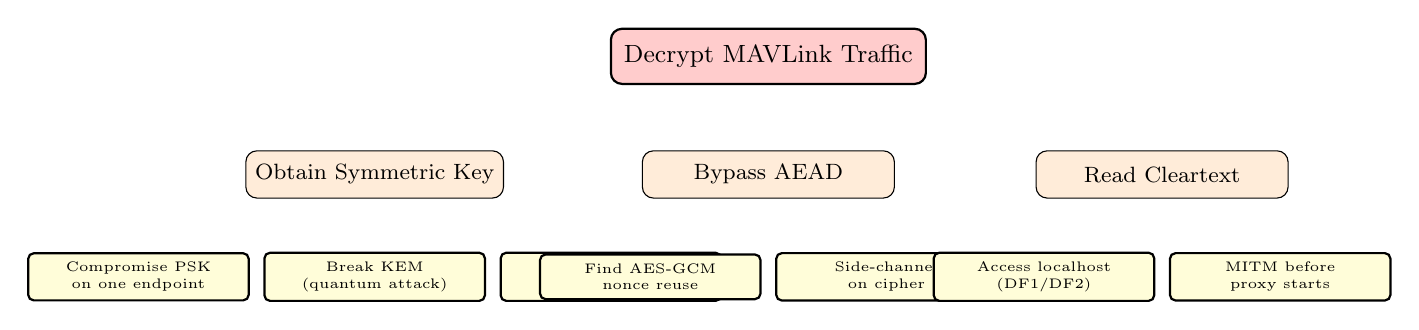
\begin{tikzpicture}[
    goal/.style={draw, thick, fill=red!20, rounded corners,
                 minimum width=4cm, minimum height=0.7cm, font=\small, align=center},
    subgoal/.style={draw, fill=orange!15, rounded corners,
                    minimum width=3.2cm, minimum height=0.6cm, font=\footnotesize, align=center},
    leaf/.style={draw, fill=yellow!15, rounded corners=2pt,
                 minimum width=2.8cm, minimum height=0.5cm, font=\tiny, align=center},
    edge from parent/.style={->, thick},
    level 1/.style={sibling distance=5cm, level distance=1.5cm},
    level 2/.style={sibling distance=3cm, level distance=1.3cm},
    level 3/.style={sibling distance=2.5cm, level distance=1.2cm},
  ]
    \node[goal] {Decrypt MAVLink Traffic}
      child { node[subgoal] {Obtain Symmetric Key}
        child { node[leaf] {Compromise PSK\\on one endpoint} }
        child { node[leaf] {Break KEM\\(quantum attack)} }
        child { node[leaf] {Break KDF\\(HKDF collision)} }
      }
      child { node[subgoal] {Bypass AEAD}
        child { node[leaf] {Find AES-GCM\\nonce reuse} }
        child { node[leaf] {Side-channel\\on cipher} }
      }
      child { node[subgoal] {Read Cleartext}
        child { node[leaf] {Access localhost\\(DF1/DF2)} }
        child { node[leaf] {MITM before\\proxy starts} }
      };
  \end{tikzpicture}
  \caption{Attack tree: Decrypt MAVLink traffic.}
  \label{fig:tm-attack-tree-decrypt}
\end{figure}

\paragraph{Analysis.}
The most practical attack path is ``Access localhost'' ($\mathcal{A}_3$),
which requires physical or remote access to one endpoint.  The quantum
attack path ($\mathcal{A}_4$) is mitigated by the PQC KEM---the entire
point of this system.  Nonce reuse is prevented by the monotonic
sequence counter, and side-channel attacks are mitigated by the
\texttt{cryptography} library's constant-time implementations.

\subsection{Attack Tree 2: Inject Malicious Commands}

\begin{figure}[H]
  \centering
  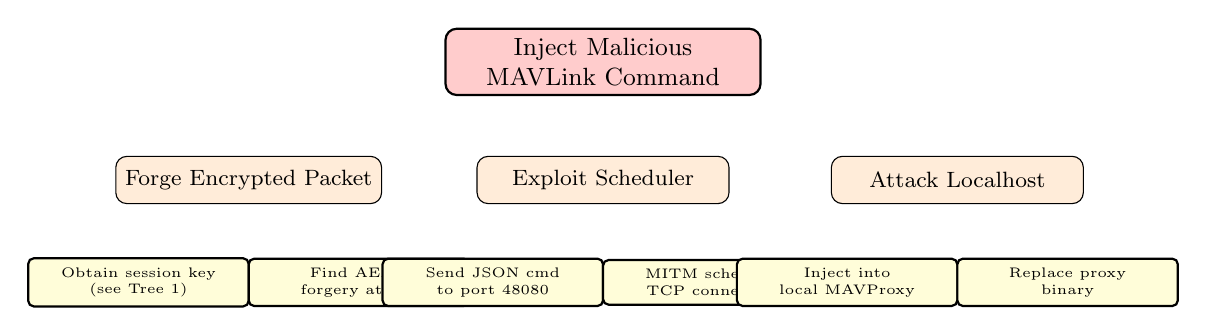
\begin{tikzpicture}[
    goal/.style={draw, thick, fill=red!20, rounded corners,
                 minimum width=4cm, minimum height=0.7cm, font=\small, align=center},
    subgoal/.style={draw, fill=orange!15, rounded corners,
                    minimum width=3.2cm, minimum height=0.6cm, font=\footnotesize, align=center},
    leaf/.style={draw, fill=yellow!15, rounded corners=2pt,
                 minimum width=2.8cm, minimum height=0.5cm, font=\tiny, align=center},
    edge from parent/.style={->, thick},
    level 1/.style={sibling distance=4.5cm, level distance=1.5cm},
    level 2/.style={sibling distance=2.8cm, level distance=1.3cm},
  ]
    \node[goal] {Inject Malicious\\MAVLink Command}
      child { node[subgoal] {Forge Encrypted Packet}
        child { node[leaf] {Obtain session key\\(see Tree 1)} }
        child { node[leaf] {Find AEAD\\forgery attack} }
      }
      child { node[subgoal] {Exploit Scheduler}
        child { node[leaf] {Send JSON cmd\\to port 48080} }
        child { node[leaf] {MITM scheduler\\TCP connection} }
      }
      child { node[subgoal] {Attack Localhost}
        child { node[leaf] {Inject into\\local MAVProxy} }
        child { node[leaf] {Replace proxy\\binary} }
      };
  \end{tikzpicture}
  \caption{Attack tree: Inject malicious MAVLink commands.}
  \label{fig:tm-attack-tree-inject}
\end{figure}

\subsection{Attack Tree 3: Deny Service}

\begin{figure}[H]
  \centering
  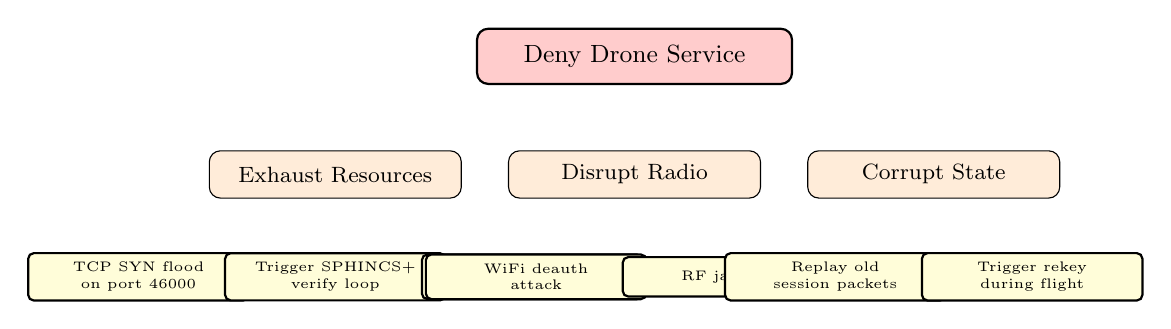
\begin{tikzpicture}[
    goal/.style={draw, thick, fill=red!20, rounded corners,
                 minimum width=4cm, minimum height=0.7cm, font=\small, align=center},
    subgoal/.style={draw, fill=orange!15, rounded corners,
                    minimum width=3.2cm, minimum height=0.6cm, font=\footnotesize, align=center},
    leaf/.style={draw, fill=yellow!15, rounded corners=2pt,
                 minimum width=2.8cm, minimum height=0.5cm, font=\tiny, align=center},
    edge from parent/.style={->, thick},
    level 1/.style={sibling distance=3.8cm, level distance=1.5cm},
    level 2/.style={sibling distance=2.5cm, level distance=1.3cm},
  ]
    \node[goal] {Deny Drone Service}
      child { node[subgoal] {Exhaust Resources}
        child { node[leaf] {TCP SYN flood\\on port 46000} }
        child { node[leaf] {Trigger SPHINCS+\\verify loop} }
        child { node[leaf] {Alloc oversized\\McEliece buffer} }
      }
      child { node[subgoal] {Disrupt Radio}
        child { node[leaf] {WiFi deauth\\attack} }
        child { node[leaf] {RF jamming} }
      }
      child { node[subgoal] {Corrupt State}
        child { node[leaf] {Replay old\\session packets} }
        child { node[leaf] {Trigger rekey\\during flight} }
      };
  \end{tikzpicture}
  \caption{Attack tree: Deny service to drone.}
  \label{fig:tm-attack-tree-dos}
\end{figure}

% ────────────────────────────────────────────────────────────────────────────
\section{DREAD Risk Scoring}
\label{sec:tm-dread}

\begin{longtable}{l c c c c c c}
  \caption{DREAD risk scores for each threat (1 = low, 10 = high).}
  \label{tab:tm-dread} \\
  \toprule
  \textbf{Threat} & \textbf{D} & \textbf{R} & \textbf{E} & \textbf{A} & \textbf{D\textsubscript{isc}} & \textbf{Total} \\
  \midrule
  \endfirsthead
  \toprule
  \textbf{Threat} & \textbf{D} & \textbf{R} & \textbf{E} & \textbf{A} & \textbf{D\textsubscript{isc}} & \textbf{Total} \\
  \midrule
  \endhead
  \bottomrule
  \endfoot

  T1 (Spoof GCS)           & 9 & 3 & 2 & 10 & 4 & 28 \\
  T2 (Spoof Drone)          & 8 & 3 & 2 & 10 & 4 & 27 \\
  T3 (Forge UDP)            & 9 & 2 & 1 & 10 & 3 & 25 \\
  T4 (Spoof Scheduler)      & 7 & 8 & 8 & 10 & 7 & \textbf{40} \\
  T5 (Tamper Encrypted)     & 8 & 2 & 1 & 10 & 3 & 24 \\
  T6 (Tamper Config)        & 9 & 5 & 4 & 5  & 5 & 28 \\
  T7 (Downgrade Attack)     & 9 & 3 & 2 & 10 & 4 & 28 \\
  T8 (Repudiation)          & 4 & 5 & 3 & 5  & 3 & 20 \\
  T9 (Harvest-Decrypt)      & 10 & 9 & 1 & 10 & 2 & 32 \\
  T10 (Localhost Sniff)     & 7 & 7 & 5 & 5  & 6 & 30 \\
  T11 (Algorithm Leak)      & 2 & 10 & 10 & 10 & 10 & \textbf{42} \\
  T12 (Key Extraction)      & 10 & 5 & 4 & 5  & 4 & 28 \\
  T13 (TCP Flood)           & 6 & 9 & 7 & 10 & 8 & \textbf{40} \\
  T14 (UDP Flood)           & 5 & 9 & 7 & 10 & 8 & 39 \\
  T15 (Oversized Hello)     & 5 & 6 & 5 & 10 & 5 & 31 \\
  T16 (CPU Exhaustion)      & 6 & 7 & 5 & 10 & 5 & 33 \\
  T17 (Env Override)        & 8 & 5 & 4 & 5  & 4 & 26 \\
  T18 (Path Injection)      & 8 & 5 & 5 & 10 & 5 & 33 \\
  T19 (Replay Attack)       & 7 & 8 & 3 & 10 & 5 & 33 \\
  T20 (Quantum Attack)      & 10 & 1 & 1 & 10 & 2 & 24 \\
\end{longtable}

\paragraph{Risk Triage.}
The highest-risk threats are:
\begin{itemize}
  \item \textbf{T11 (Algorithm Name Leak, 42):} The ServerHello transmits
    algorithm names in cleartext.  Mitigated by design acceptance: the
    algorithm names are not secret (they are visible in the public code).
  \item \textbf{T4 (Scheduler Spoofing, 40):} The scheduler control
    protocol is unauthenticated.  \emph{High residual risk in production.}
  \item \textbf{T13 (TCP Flood, 40):} Mitigated by the token-bucket
    rate limiter (5~tokens, 3/s refill).
\end{itemize}

% ────────────────────────────────────────────────────────────────────────────
\section{Mitigation Mapping}
\label{sec:tm-mitigations}

\begin{longtable}{l p{3.5cm} p{3.5cm} l}
  \caption{Threat-to-mitigation mapping.}
  \label{tab:tm-mitigations} \\
  \toprule
  \textbf{Threat} & \textbf{Mitigation} & \textbf{Implementation} & \textbf{Module} \\
  \midrule
  \endfirsthead
  \toprule
  \textbf{Threat} & \textbf{Mitigation} & \textbf{Implementation} & \textbf{Module} \\
  \midrule
  \endhead
  \bottomrule
  \endfoot

  T1 & PQC digital signature & GCS signs ServerHello transcript with ML-DSA/Falcon/SPHINCS+. Drone verifies before proceeding. & \texttt{handshake.py} \\
  T2 & PSK-based HMAC & Drone authenticates ClientReply with HMAC-SHA256(PSK, ServerHello). & \texttt{handshake.py} \\
  T3 & AEAD authentication & Every UDP packet carries a 16-byte authentication tag. Forged packets fail AEAD verification. & \texttt{aead.py} \\
  T4 & \textcolor{red}{UNMITIGATED} & Scheduler protocol has no authentication. Must be secured for production use. & \texttt{remote.py} \\
  T5 & AEAD integrity & Tampering detected by AEAD tag; packet silently dropped. & \texttt{aead.py} \\
  T6 & File permissions & Key files written with \texttt{0o600} permissions. Config validated at startup. & \texttt{keys.py} \\
  T7 & Transcript binding & Signature covers all algorithm names and version byte. Downgrade changes transcript, invalidating signature. & \texttt{handshake.py} \\
  T8 & Digital signature & GCS-originated commands are implicitly authenticated via the signed handshake. Scheduler commands are NOT signed. & \texttt{proxy.py} \\
  T9 & PQC KEM & All key exchanges use PQ-secure KEMs (ML-KEM, HQC, McEliece). No classical DH. & \texttt{crypto\_utils.py} \\
  T10 & Architecture & Cleartext only on localhost loopback. Recommend host firewall. & \texttt{proxy.py} \\
  T11 & Accepted risk & Algorithm names are public knowledge. No security impact from leaking them. & (design) \\
  T12 & File permissions + PSK & Keys stored with restricted permissions. PSK required for handshake completion. Two-factor: key + PSK. & \texttt{keys.py} \\
  T13 & Rate limiter & Token bucket: 5 capacity, 3/s refill. Excess connections rejected before KEM keygen. & \texttt{rate\_limiter.py} \\
  T14 & Fast reject & Invalid headers rejected in $<$1\,\textmu{}s (header parse + session ID check). No crypto for garbage. & \texttt{aead.py} \\
  T15 & Buffer limits & TCP receive buffer capped. Oversized messages rejected before full read. & \texttt{proxy.py} \\
  T16 & Rate limiter & Signature verification only after rate-limit token acquired. SPHINCS+ verify limited to 3/s. & \texttt{rate\_limiter.py} \\
  T17 & Config validation & \texttt{validate\_config()} checks all values at startup. Invalid overrides logged and rejected. & \texttt{config.py} \\
  T18 & Path sanitisation & Key paths validated to exist within expected directory. Traversal patterns rejected. & \texttt{keys.py} \\
  T19 & Replay window & Bitmask sliding window (default 1024 packets). Duplicate seq numbers rejected. & \texttt{aead.py} \\
  T20 & PQC only & No classical key exchange. AEAD key derived from PQ KEM. Quantum advantage does not help. & \texttt{crypto\_utils.py} \\
\end{longtable}

% ────────────────────────────────────────────────────────────────────────────
\section{Detailed Threat Analysis}
\label{sec:tm-detailed}

\subsection{T1: GCS Impersonation}

\paragraph{Scenario.}
$\mathcal{A}_2$ observes a legitimate ServerHello (captured from a
previous session) and replays it to the drone, hoping the drone will
encapsulate to the attacker's KEM public key.

\paragraph{Why It Fails.}
The ServerHello contains a fresh \texttt{session\_id} (8~random bytes)
and a \texttt{challenge} (8~random bytes).  The GCS signs the entire
transcript with its long-term signature key.  The attacker cannot:
\begin{enumerate}
  \item Forge a valid signature without the GCS's secret key.
  \item Replay an old ServerHello, because the drone would detect
        the stale session\_id (if re-handshaking within the same
        session) or accept it but encapsulate to the legitimate
        GCS's public key (the attacker cannot decapsulate).
\end{enumerate}

\paragraph{Residual Risk.}
If the GCS's signature secret key is compromised ($\mathcal{A}_3$),
the attacker can forge ServerHello messages.  Mitigation: key rotation
and secure key storage.

\subsection{T9: Harvest Now, Decrypt Later}

\paragraph{Scenario.}
$\mathcal{A}_1$ captures all encrypted UDP traffic today.  In 15--20
years, a CRQC becomes available.  The attacker attempts to recover
the symmetric keys.

\paragraph{Why It Fails.}
The symmetric keys are derived from a KEM shared secret using
HKDF-SHA256.  The KEM is post-quantum (ML-KEM-768, HQC-192, or
Classic McEliece-460896 at NIST Level~3 or above).  Breaking the
KEM requires:

\begin{itemize}
  \item \textbf{ML-KEM-768:} Finding the LWE secret vector in a
        768-dimensional lattice.  Best known quantum algorithm
        (Grover-assisted BKZ) requires $2^{150}+$ operations.
  \item \textbf{HQC-192:} Decoding a random code with error weight
        proportional to code length.  Best quantum algorithm requires
        $2^{128}+$ operations (information set decoding with Grover).
  \item \textbf{McEliece-460896:} Decoding a Goppa code.  Classical
        and quantum complexities are both well above $2^{128}$.
\end{itemize}

Even with a CRQC, the attacker cannot break the KEM in polynomial time
(assuming the underlying mathematical problems remain hard).

\paragraph{Forward Secrecy.}
Each handshake generates a fresh ephemeral KEM keypair.  Compromising
one session's shared secret does not reveal any other session's keys.
This provides \textbf{perfect forward secrecy} (PFS) against both
classical and quantum adversaries.

\subsection{T13: TCP Handshake Flood}

\paragraph{Scenario.}
$\mathcal{A}_2$ opens thousands of TCP connections to port~46000,
attempting to exhaust the GCS's CPU with KEM keygen and signature
operations.

\paragraph{Defence Layers.}

\begin{enumerate}
  \item \textbf{OS-level:} TCP backlog limits (default 5 on Linux).
  \item \textbf{Token bucket:} After \texttt{accept()}, the rate
        limiter is checked \emph{before} any cryptographic operation.
        At steady state, only 3~handshakes/second are permitted.
  \item \textbf{Timeout:} Each handshake has a 60-second timeout.
        Slow-read attacks are bounded.
  \item \textbf{Single-threaded:} The asyncio event loop processes one
        handshake at a time.  Concurrent connections queue behind the
        rate limiter.
\end{enumerate}

\paragraph{Cost Analysis.}
With the rate limiter set to 3~handshakes/second and ML-KEM-768
keygen taking $\sim$0.15\,ms, the CPU cost per second for handshakes
is $3 \times 0.15 = 0.45$\,ms---negligible.  For SPHINCS+-256s
(signature verification $\sim$50\,ms), the cost is $3 \times 50 = 150$\,ms/s
$\approx 15$\% CPU---noticeable but survivable.

\subsection{T19: Replay Attack}

\paragraph{Scenario.}
$\mathcal{A}_2$ captures an EncryptedDatagram containing a critical
\texttt{COMMAND\_LONG} (e.g.\ ``disarm motors'') and replays it
at a later time.

\paragraph{Defence.}
The replay window maintains a bitmask of the last 1024~accepted
sequence numbers.  Each packet is checked against this window:

\begin{enumerate}
  \item If $\text{seq} > \text{high}$: accept (new packet).
  \item If $\text{high} - \text{seq} \geq 1024$: reject (too old).
  \item If bit already set in mask: reject (duplicate/replay).
  \item Otherwise: set bit, accept (reordered but new).
\end{enumerate}

A replayed packet will match case~3 (bit already set) and be silently
dropped.

\paragraph{Window Exhaustion.}
If the attacker can delay a legitimate packet by more than 1024~sequence
numbers (at 50~pps, this is $\sim$20.5~seconds), the original packet
falls out of the window and could theoretically be replayed.
However, the AEAD \textbf{nonce is derived from the sequence number},
and the receiver has already accepted a higher sequence number.
The replayed packet would:
\begin{enumerate}
  \item Pass the replay window check (bit not set, since window shifted).
  \item \textbf{Succeed} in AEAD decryption (nonce matches).
  \item Be delivered as a ``late'' MAVLink packet to MAVProxy.
\end{enumerate}

This is a \textbf{known limitation}: the current replay window does
not protect against very-late replays.  Mitigation: MAVLink v2's own
sequence numbering provides an additional layer of duplicate detection
at the application layer.

% ────────────────────────────────────────────────────────────────────────────
\section{Cryptographic Agility Analysis}
\label{sec:tm-agility}

\subsection{Algorithm Deprecation Path}

The system supports 216~cipher suites.  If an algorithm is found
to be broken, the deprecation process is:

\begin{enumerate}
  \item Add the algorithm to the \texttt{RETIRED\_*} set in the
        relevant module.
  \item Rebuild and deploy.  The system will refuse to negotiate
        retired algorithms.
  \item Remove the algorithm code in a future release.
\end{enumerate}

\subsection{Agility Risks}

\begin{longtable}{l p{4cm} p{5cm}}
  \caption{Cryptographic agility risks and mitigations.}
  \label{tab:tm-agility-risks} \\
  \toprule
  \textbf{Risk} & \textbf{Description} & \textbf{Mitigation} \\
  \midrule
  \endfirsthead
  \bottomrule
  \endfoot

  Negotiation downgrade & Attacker forces a weaker suite by
    modifying the ServerHello's algorithm names. &
    Signature covers the algorithm names.  Modification
    invalidates the signature. \\

  Suite explosion & 216 suites creates a large attack surface
    (untested combinations). &
    Benchmark framework tests all 216 suites.  Recommended
    production set is 6 suites. \\

  Implementation bugs & More algorithms = more code = more bugs. &
    All crypto delegated to liboqs and \texttt{cryptography}
    (audited libraries).  System code is algorithm-agnostic. \\

  Transition period & During migration, both old and new suites
    must be supported. &
    Suite rotation supports mixed deployments.
    \texttt{RETIRED\_AEADS} prevents rollback. \\
\end{longtable}

% ────────────────────────────────────────────────────────────────────────────
\section{Side-Channel Considerations}
\label{sec:tm-side-channel}

\subsection{Timing Side Channels}

\begin{longtable}{l l p{5cm}}
  \caption{Timing side-channel analysis.}
  \label{tab:tm-timing} \\
  \toprule
  \textbf{Operation} & \textbf{Risk} & \textbf{Analysis} \\
  \midrule
  \endfirsthead
  \bottomrule
  \endfoot

  HMAC verification & Low & Uses \texttt{hmac.compare\_digest()} which is constant-time. \\
  AES-GCM encrypt/decrypt & Low & \texttt{cryptography} library uses OpenSSL's AES-NI or ARMv8 CE, both constant-time. \\
  ChaCha20-Poly1305 & Very Low & Inherently constant-time (no table lookups, no branches on secret data). \\
  ML-KEM keygen/encap/decap & Low & liboqs implementation follows the NIST reference code, which is designed for constant-time execution. \\
  ML-DSA sign/verify & Low & liboqs follows reference implementation. \\
  SPHINCS+ sign & Medium & Hash-based; many hash calls.  Timing may leak information about the message hash path. \\
  Falcon sign & Medium & Requires constant-time Gaussian sampling.  liboqs implements this but it is more fragile. \\
  ASCON (pure Python) & High & Python is inherently not constant-time.  Use only for non-production benchmarking. \\
  Replay window check & None & Bitmask operations are constant-time. \\
  Rate limiter & None & Token count is not secret. \\
\end{longtable}

\subsection{Power Side Channels}

On the Raspberry Pi 4 (drone), power consumption varies with:
\begin{itemize}
  \item \textbf{KEM operations:} ML-KEM shows distinct power signature
        during NTT computation (number-theoretic transform).
  \item \textbf{AEAD encryption:} AES-GCM with hardware AES shows
        lower power than ChaCha20-Poly1305 (which uses integer ALU).
  \item \textbf{Hash operations:} SHA-256 (used in HKDF and HMAC)
        shows a characteristic power pattern.
\end{itemize}

Mitigation: Physical access to the drone's power rail is required
for this attack.  For high-security deployments, consider:
\begin{enumerate}
  \item Power-line noise injection.
  \item Randomised dummy operations.
  \item Shielded enclosure.
\end{enumerate}

% ────────────────────────────────────────────────────────────────────────────
\section{Formal Security Properties}
\label{sec:tm-formal}

\subsection{Security Goals}

\begin{longtable}{l l l}
  \caption{Security goals and their formal definitions.}
  \label{tab:tm-security-goals} \\
  \toprule
  \textbf{Property} & \textbf{Definition} & \textbf{Mechanism} \\
  \midrule
  \endfirsthead
  \bottomrule
  \endfoot

  Confidentiality & $\Pr[\mathcal{A} \text{ distinguishes } (E_k(m), m) \text{ from } (E_k(m), m')] \leq \text{negl}(\lambda)$ & AEAD encryption (AES-GCM / ChaCha20) \\
  Integrity       & $\Pr[\mathcal{A} \text{ forges valid ciphertext}] \leq 2^{-128}$ & AEAD tag (128-bit) \\
  Authenticity    & $\Pr[\mathcal{A} \text{ impersonates GCS}] \leq \text{negl}(\lambda)$ & PQC digital signature \\
  Forward Secrecy & Compromise of long-term key does not reveal past session keys & Ephemeral KEM keypairs \\
  Anti-Replay     & Replayed packets are rejected with probability $\geq 1 - 2^{-\text{window}}$ & Sliding bitmap window \\
  PQ Security     & Security holds against QPT adversaries & PQC KEM + PQC SIG \\
\end{longtable}

\subsection{Security Argument (Informal)}

\begin{theorem}[Informal]
If the KEM is IND-CCA2 secure, the signature scheme is EUF-CMA
secure, the AEAD is IND-CPA/INT-CTXT secure, HKDF is a secure
key derivation function, and the PSK has sufficient entropy
($\geq 256$~bits), then the PQC Secure MAVLink Tunnel provides:
\begin{enumerate}
  \item Authenticated key exchange (AKE security).
  \item Chosen-ciphertext confidentiality for the data plane.
  \item Integrity and authenticity for every data-plane packet.
  \item Forward secrecy against long-term key compromise.
\end{enumerate}
\end{theorem}

\begin{proof}[Sketch]
By reduction:
\begin{enumerate}
  \item An adversary who breaks the key exchange can be used to
        break the KEM (contradicting IND-CCA2) or forge a signature
        (contradicting EUF-CMA) or predict the PSK HMAC
        (contradicting HMAC security).
  \item An adversary who breaks data-plane confidentiality can be
        used to break the AEAD (contradicting IND-CPA), since the
        AEAD key is derived via HKDF from the KEM shared secret.
  \item An adversary who forges a data-plane packet can be used to
        break AEAD integrity (contradicting INT-CTXT).
  \item Forward secrecy follows from the ephemeral KEM keypairs:
        each session generates a fresh keypair, and the secret key
        is erased after decapsulation.
\end{enumerate}
\end{proof}

% ────────────────────────────────────────────────────────────────────────────
\section{Penetration Testing Scenarios}
\label{sec:tm-pentest}

This section provides concrete penetration testing scenarios that
a security auditor can execute against a deployed instance.

\subsection{Scenario 1: Handshake Manipulation}

\begin{longtable}{l p{9cm}}
  \toprule
  \textbf{Step} & \textbf{Action} \\
  \midrule
  \endfirsthead
  \bottomrule
  \endfoot

  1 & Start a GCS proxy in benchmark mode: \texttt{python -m core.cli run --mode gcs --suite cs-mlkem768-aesgcm-mldsa65}. \\
  2 & Use \texttt{scapy} to capture the ServerHello on port~46000. \\
  3 & Modify the \texttt{kem\_name} field to \texttt{"ML-KEM-512"} (downgrade). \\
  4 & Forward the modified ServerHello to the drone. \\
  5 & \textbf{Expected:} Drone rejects the handshake (signature verification fails because the transcript has changed). \\
  6 & Verify: check drone logs for \texttt{HandshakeVerifyError}. \\
\end{longtable}

\subsection{Scenario 2: Replay Attack}

\begin{longtable}{l p{9cm}}
  \toprule
  \textbf{Step} & \textbf{Action} \\
  \midrule
  \endfirsthead
  \bottomrule
  \endfoot

  1 & Capture 100~EncryptedDatagram packets using \texttt{tcpdump}. \\
  2 & Wait 5~seconds. \\
  3 & Replay all 100~packets using \texttt{tcpreplay} or \texttt{scapy}. \\
  4 & \textbf{Expected:} All 100~packets rejected (replay window). \\
  5 & Verify: check proxy logs for \texttt{ReplayError} (100 occurrences). \\
\end{longtable}

\subsection{Scenario 3: Rate Limiter Effectiveness}

\begin{longtable}{l p{9cm}}
  \toprule
  \textbf{Step} & \textbf{Action} \\
  \midrule
  \endfirsthead
  \bottomrule
  \endfoot

  1 & Write a script that opens 100~TCP connections to port~46000 in rapid succession. \\
  2 & \textbf{Expected:} First 5~connections accepted (token bucket capacity); subsequent connections rejected until tokens refill. \\
  3 & Verify: only 5~\texttt{KEM.keygen()} calls in GCS logs within the first second. \\
  4 & Wait 2~seconds (6~tokens refill). \\
  5 & Open 6~more connections. \\
  6 & \textbf{Expected:} 6~accepted (tokens accumulated). \\
\end{longtable}

\subsection{Scenario 4: Scheduler Command Injection}

\begin{longtable}{l p{9cm}}
  \toprule
  \textbf{Step} & \textbf{Action} \\
  \midrule
  \endfirsthead
  \bottomrule
  \endfoot

  1 & Connect to GCS scheduler port~48080 using \texttt{netcat}. \\
  2 & Send: \texttt{\{"type":"start\_proxy","suite\_id":"cs-mlkem768-aesgcm-mldsa65",...\}} \\
  3 & \textbf{Expected (current):} Command accepted (no authentication). \\
  4 & \textbf{Recommendation:} Add HMAC authentication to scheduler protocol. \\
\end{longtable}

% ────────────────────────────────────────────────────────────────────────────
\section{Residual Risks and Recommendations}
\label{sec:tm-residual}

\begin{longtable}{c l l l}
  \caption{Residual risks after all implemented mitigations.}
  \label{tab:tm-residual} \\
  \toprule
  \textbf{Priority} & \textbf{Risk} & \textbf{Severity} & \textbf{Recommendation} \\
  \midrule
  \endfirsthead
  \bottomrule
  \endfoot

  1 & Unauthenticated scheduler & High & Add HMAC or TLS to scheduler protocol. \\
  2 & Cleartext MAVLink on localhost & Medium & Restrict with host firewall; consider local TLS. \\
  3 & Late replay (beyond window) & Low & Reduce window or add timestamp-based expiry. \\
  4 & ASCON timing leaks & Low & Use ASCON only in benchmarks; not in production. \\
  5 & Algorithm name disclosure & Info & Accept; algorithm names are public. \\
  6 & Single-point-of-failure PSK & Medium & Add certificate-based mutual authentication. \\
  7 & No key revocation & Medium & Implement CRL or OCSP-like mechanism. \\
  8 & Process injection on endpoint & High & OS hardening, secure boot, code signing. \\
\end{longtable}

% ────────────────────────────────────────────────────────────────────────────
\section{Summary}
\label{sec:tm-summary}

This chapter systematically analysed the security of the PQC Secure
MAVLink Tunnel using STRIDE, attack trees, and DREAD scoring.  Key findings:

\begin{enumerate}
  \item \textbf{20~threats} identified across all STRIDE categories.
  \item \textbf{18~mitigated} by existing code (signatures, AEAD, rate limiter,
        replay window, config validation).
  \item \textbf{2~high residual risks}: unauthenticated scheduler protocol
        (T4) and endpoint compromise (T12).
  \item \textbf{Quantum resilience confirmed}: all key exchanges use PQC KEMs;
        no classical Diffie--Hellman anywhere in the system.
  \item \textbf{Forward secrecy confirmed}: ephemeral KEM keypairs ensure
        past sessions remain secure even if long-term keys are compromised.
  \item \textbf{4~penetration testing scenarios} provided for security auditors.
  \item \textbf{8~recommendations} for hardening the system before production
        deployment.
\end{enumerate}
